%Organize this section according to the rules defined in the project description. 
% to do add notification on student registration and to post anew internship us

\subsection{External Interface Requirements}
    \subsubsection{User Interfaces}
    We prefer not to tie our design to any guidelines so early in the project, so we will probably give some snippets of the user interfaces in the DD. However, the principles that will guide our design will be clarity and minimalism. We believe that at the basis of a well working web application there must be a nice user interface. We are also convinced that being minimal and simple looking is a plus for a web application since a confusing user interface is one of the biggest reasons why users dislike a certain website and prefer another to it.

    \subsubsection{Hardware Interfaces}
    Being our project a web application there are not many hardware requirements. From the client side perspective the only request is about the size of the monitor. Indeed the website is going to be developed for desktop view exclusively. Apart of that, any laptop with a stable internet access will suffice. On the server side, any kind of setup is acceptable since our website does not have specific requirements for special computing power or similar capabilities.

    \subsubsection{Software Interfaces}
    From the perspective of software interfaces, there is only one standard requirement: the platform must be compatible with all the latest stable versions of the major web browsers
    
    \subsubsection{Communication Interfaces}
    S\&C communicates important information to users through notifications on the website.
    
    \begin{enumerate}
        \item  \textbf{Push Notifications}: notifications created when a company posted an internship or a student with the right skill set for an internship position becomes available on the platform
        \item \textbf{Real Time Notifications}: notifications created when an action is performed by a user to let him/her know that it has been successful or not
    \end{enumerate}

% --------------------------------------
\newpage
\subsection{Functional Requirements}
    The listed requirements are in the form suggested by IEEE\cite{502838}: 
    \newline
    \newline
    [Condition][Subject][Action][Object][Constraints on the Action] \\
    \subsubsection*{Users:}
        \begin{enumerate}[label=\textbf{R\arabic*}]
            \item S\&C shall allow users to sign up.                  
            \item S\&C shall allow users to fill in their profile information when signing up.
            \item S\&C shall allow users to log in.                   
            \item S\&C shall allow users to log out.                  
            \item S\&C shall allow users to update their profile information. 
            \item S\&C shall allow users to examine their own internships.
            \end{enumerate}
        
    \subsubsection*{Students:}
        \begin{enumerate}[label=\textbf{R\arabic*},resume]
            \item S\&C shall allow students to examine open internship positions. % To check
            \item S\&C shall allow students to examine their own applications.
            \item S\&C shall allow students to search for a specific kind of internship position.  
            \item S\&C shall allow students to apply for an internship position.
            \item If an internship position suitable for a student is opened, S\&C shall notify the student.
            \item When a student searches for an internship, S\&C shall list the different positions aligned with the student's profile.         
        \end{enumerate}
    
    \subsubsection*{Applications:}
        \begin{enumerate}[label=\textbf{R\arabic*},resume]
            \item If an application has been accepted by a company, S\&C shall allow the student who made the application to confirm or refuse the internship.
            \item If a company signals that it needs an assessment of the students' skills, S\&C shall allow the company to schedule an interview.
            \item After an interview has been scheduled, S\&C shall allow the student to access the link and see the date of the meeting.
            \item S\&C shall allow the students to see the status of their applications.
        \end{enumerate}
    
    \subsubsection*{Companies:}
        \begin{enumerate}[label=\textbf{R\arabic*},resume]
            \item S\&C shall allow companies to open and examine its internship positions.
            \item S\&C shall allow companies to accept or reject applications for their internship positions.
            \item S\&C shall allow companies to close internship positions.
            \item If a new profile of a student who could interest a company becomes available on the platform, S\&C shall notify the company.
        \end{enumerate}
    
    \subsubsection*{Communication during the internship:}
         \begin{enumerate}[label=\textbf{R\arabic*},resume]
            \item S\&C shall allow companies to leave private notes to students who are doing an internship with it.
            \item S\&C shall allow companies to send news about the internship to the students who participate in it.
            \item S\&C shall allow both parties to communicate problems in a specific space of the website.
        \end{enumerate}
    
    \subsubsection*{Feedback and Suggestions:}
        \begin{enumerate}[label=\textbf{R\arabic*},resume]
            \item S\&C shall allow students who took an internship with a company to rate the internship and vice versa.
            \item S\&C shall allow students who took an internship with a company to give suggestions to the company and vice versa.
            \item S\&C shall allow companies to send news about the internship to students who are carrying it out.
            \item S\&C shall allow both parties involved in an internship to make complaints in a dedicated space.
        \end{enumerate}
        
    \subsubsection*{Universities:}
        \begin{enumerate}[label=\textbf{R\arabic*},resume]
            \item S\&C shall allow universities to monitor the status of the internship of their students.
            \item S\&C shall allow universities to see details of the internships of their students.
        \end{enumerate}
        
\newpage

\subsection{Use Cases and Use Case Diagrams}

    This section is dedicated to use cases and use case diagrams. In order to be as clear as possible here is the general schema of the use cases and their links with the actors. 
\\
\\
\\
\\
\\
\\
\\
\\
\\
    \begin{figure}[h!]
                \centering
                    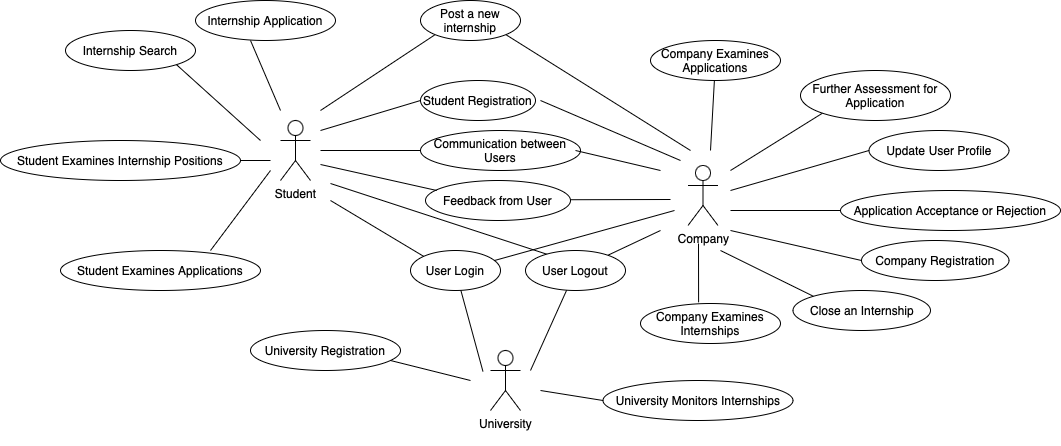
\includegraphics[width=1\textwidth]{RASD/Images/GeneralSchemaUS.drawio.png}
                \label{fig:example}
            \end{figure}
\\
\\
\\
\\
In the following pages all the use cases along with their diagrams are listed.
\newpage
    \subsubsection{User Use Cases}
    
        \begin{enumerate}[label=\textbf{[US\arabic*]}, left = 0pt, align = left]
            % -- US1 --                                                      
            \item \textbf{User Login}
            
            \begin{longtable}{|l|p{11cm}|}  
                \hline
                \textbf{Name} & 
                    \textbf{User Login} \\
                \hline
                
                \textbf{Actors} & 
                    \begin{enumerate}[label=\textbullet, itemsep=0em]
                        \item User
                    \end{enumerate} \\
                \hline
                
                \textbf{Entry Condition} & 
                    \begin{enumerate}[label=\textbullet, itemsep=0em]
                        \item The user wants to log in;
                        \item The user has an account and is on the main page of S\&C.
                    \end{enumerate} \\
                \hline
                
                \textbf{Event Flow} &
                    \begin{enumerate}[label=\arabic*., itemsep=0.2em]
                        \item The user presses the "Login" button;
                        \item S\&C redirects the user to the login page;
                        \item The user types the email in the corresponding form field;
                        \item The user types the password in the corresponding form field;
                        \item The user presses the "Log in" button;
                        \item S\&C validates the data;
                        \item S\&C redirects the user to the homepage of S\&C.
                    \end{enumerate} \\
                \hline
                
                \textbf{Exit Condition} & 
                    The user logs into his/her profile. \\
                \hline
                
                \textbf{Exceptions} &
                    \begin{enumerate}[label=\arabic*., itemsep=0.1em]
                        \item A user with the entered email doesn't exists.
                            \begin{itemize}[label=\textbullet, itemsep=0em]
                                \item In that case, S\&C will display an error message on the screen.
                            \end{itemize}
                        \item The entered password and the stored password do not match.
                            \begin{itemize}[label=\textbullet, itemsep=0em]
                                \item In that case, S\&C will display an error message on the screen.
                            \end{itemize}
                    \end{enumerate} \\
                \hline
                
            \end{longtable}

            \newpage 
            \begin{figure}[h!]
                \centering
                    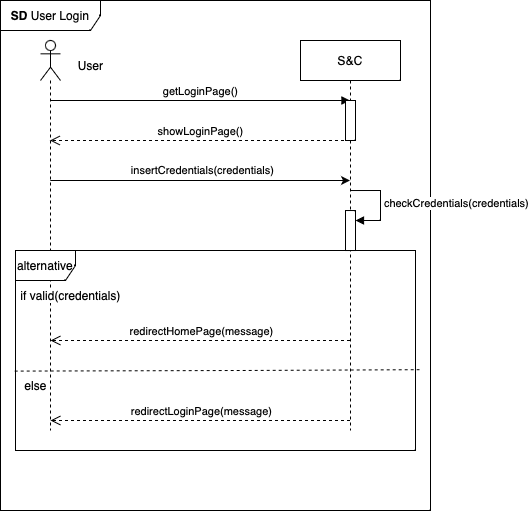
\includegraphics[width=1\textwidth]{RASD/Images/UseCases/US01_UserLogin.drawio.png}
                \label{fig:example}
            \end{figure}
  
            % -- US2 --                                                     
            \newpage
            \item \textbf{User Logout}
            
            \begin{longtable}{|l|p{11cm}|}  
                \hline
                \textbf{Name} & 
                    \textbf{User Logout} \\
                \hline
                
                \textbf{Actors} & 
                    \begin{enumerate}[label=\textbullet, itemsep=0em]
                        \item User
                    \end{enumerate} \\
                \hline
                
                \textbf{Entry Condition} & 
                    \begin{enumerate}[label=\textbullet, itemsep=0em]
                        \item The user wants to log out;
                        \item The user has an account, is logged in, and is on his/her homepage.
                    \end{enumerate} \\
                \hline
                
                \textbf{Event Flow} &
                    \begin{enumerate}[label=\arabic*., itemsep=0.2em]
                        \item The user presses the "Logout" button;
                        \item S\&C redirects the user to the login page and displays a Success Message;
                    \end{enumerate} \\
                \hline
                
                \textbf{Exit Condition} & 
                    The user logs out his/her profile. \\
                \hline
                
                \textbf{Exceptions} &
                    \begin{enumerate}[label=\arabic*., itemsep=0.1em]
                        \item The user doesn't have an account.
                            \begin{itemize}[label=\textbullet, itemsep=0em]
                                \item In that case, S\&C will display an error message on the screen.
                            \end{itemize}
                    \end{enumerate} \\
                \hline
                
            \end{longtable}

            \newpage
            \begin{figure}[h!]
                \centering
                    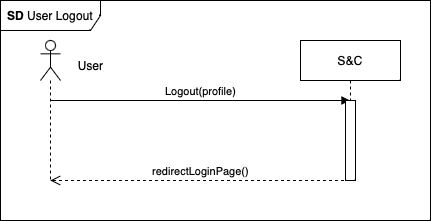
\includegraphics[width=1\textwidth]{RASD/Images/UseCases/US02_UserLogout.drawio.png}
                \label{fig:example}
            \end{figure}

            % -- US3 --                                                      
            \newpage
            
            \item \textbf{Update User Profile}
            
            \begin{longtable}{|l|p{11cm}|}  
                \hline
                \textbf{Name} & 
                    \textbf{Update User Profile} \\
                \hline
                
                \textbf{Actors} & 
                    \begin{enumerate}[label=\textbullet, itemsep=0em]
                        \item User
                    \end{enumerate} \\
                \hline

                \textbf{Entry Condition} & 
                    \begin{enumerate}[label=\textbullet, itemsep=0em]
                        \item The user decides to modify his/her profile;
                        \item The user has an account, is logged in, and is on his homepage.
                    \end{enumerate} \\
                \hline
                
                \textbf{Event Flow} &
                    \begin{enumerate}[label=\arabic*., itemsep=0.2em]
                        \item The user presses the "Edit Profile" button;
                        \item S\&C redirects the user to the personal profile page;
                        \item The user choose which information modify;
                        \item The user presses the "Modify" button on the right of the desired category;
                        \item The user modifies the data;
                        \item The user presses the "Apply Changes" button;
                        \item S\&C validates the data;
                        \item S\&C redirects the user to the homepage of S\&C.
                    \end{enumerate} \\
                \hline
                
                \textbf{Exit Condition} & 
                    The user's profile is successfully updated and saved in the system. \\
                \hline
                
                \textbf{Exceptions} &
                    \begin{enumerate}[label=\arabic*., itemsep=0.1em]
                        \item Missing Required Fields:
                            \begin{itemize}[label=\textbullet, itemsep=0em]
                                \item If any mandatory fields are left empty, S\&C will display an error message.
                            \end{itemize}
                        \item Invalid Data Format:
                            \begin{itemize}[label=\textbullet, itemsep=0em]
                                \item If at least one data is invalid, an error message is displayed;
                            \end{itemize}     
                    \end{enumerate} \\
                \hline
                
            \end{longtable}
        
            \newpage          
            \begin{figure}[h!]
                \centering
                    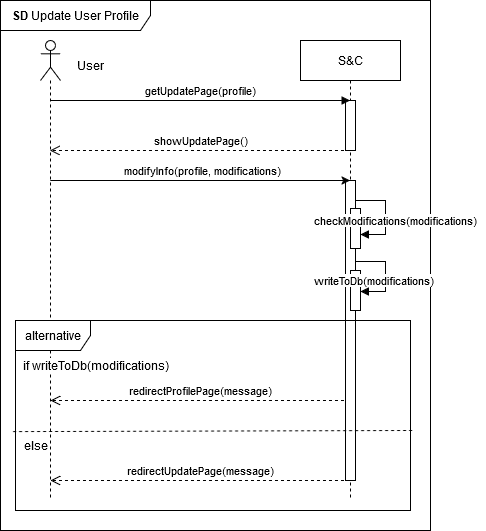
\includegraphics[width=1\textwidth]{RASD/Images/UseCases/US03_UserUpdate.drawio.png}
                \label{fig:example}
            \end{figure}

        \end{enumerate}

    % -----------------------------------
    \newpage
    \subsubsection{Student Use Cases}
    
        \begin{enumerate}[label=\textbf{[US\arabic*]}, left = 0pt, align = left, resume]
            % -- US4 --    
            \item \textbf{Student Registration}
            
            \begin{longtable}{|l|p{11cm}|}  
                \hline
                \textbf{Name} & 
                    \textbf{Student Registration} \\
                \hline
                
                \textbf{Actors} & 
                    \begin{enumerate}[label=\textbullet, itemsep=0em]
                        \item Student;
                        \item Company.
                    \end{enumerate} \\
                \hline
                
                \textbf{Entry Condition} & 
                    The student does not have an account and is on the main page of S\&C. \\
                \hline
                
                \textbf{Event Flow} &
                    \begin{enumerate}[label=\arabic*., itemsep=0.2em]
                        \item The student presses the "Register as Student" button;
                        \item S\&C redirects the student to the register page;
                        
                        \item The student types the Email in the corresponding form field;
                        \item The student types the password in the corresponding form field;
                        \item The student types the confirm password in the corresponding form field;
                        
                        \item The student enters the \textit{Basic Information} in the corresponding form field:
                        \begin{itemize}[label=\textbullet, itemsep=0em]
                            \item Full name;
                            \item Phone number;
                            \item Profile picture (not mandatory);
                            \item Location for location-based internships.
                        \end{itemize}
                        
                        \item The student enters the \textit{Academic Information}:
                        \begin{itemize}[label=\textbullet, itemsep=0em]
                            \item University name;
                            \item Degree program;
                            \item GPA (not mandatory);
                            \item Graduation year (not mandatory).
                        \end{itemize}
                        
                        \item The student types the Skills;
                        \item The student uploads the \textit{CV};
                        \item The student types the \textit{Languages Spoken}.
                        
                        \item The student presses the "Subscribe" button;
                        \item S\&C validates the data;
                        \item S\&C creates the student's account;
                        \item S\&C redirects the student to the homepage of S\&C.
                        \item S\&C identifies the internships that match the student's profile based on skills, academic background, and location;
                        \item S\&C sends notifications to companies offering internships that match the student's profile.
                    \end{enumerate} \\
                \hline
                
                \textbf{Exit Condition} & 
                    The student's account is created, and they are logged in. \\
                \hline
                
                \textbf{Exceptions} &
                    \begin{enumerate}[label=\arabic*., itemsep=0.1em]
                        \item The student provides invalid data (e.g., invalid email format, duplicate email address, mismatched passwords).
                            \begin{itemize}[label=\textbullet, itemsep=0em]
                                \item S\&C validates the input and detects the invalid data.
                                \item S\&C displays an error message explaining the specific validation errors.
                                \item The student must correct the errors and resubmit the form
                            \end{itemize}
                    \end{enumerate} \\
                \hline
            \end{longtable}
            
            \newpage
            \begin{figure}[h!]
                \centering
                    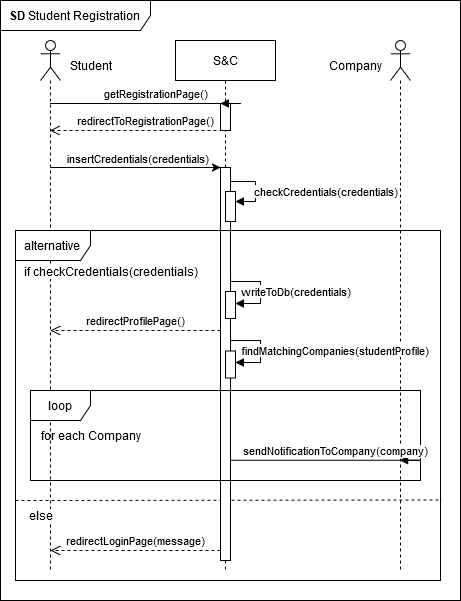
\includegraphics[width=1\textwidth]{RASD/Images/UseCases/US04_StudentRegistration.drawio.png}
                \label{fig:example}
            \end{figure}           
            
            % -- US5 --
            \newpage
            \item \textbf{Internship Search}
            
            \begin{longtable}{|l|p{11cm}|}  
                \hline
                \textbf{Name} & 
                    \textbf{Internship Search} \\
                \hline
                
                \textbf{Actors} & 
                    \begin{enumerate}[label=\textbullet, itemsep=0em]
                        \item Student
                    \end{enumerate} \\
                \hline
               
                \textbf{Entry Condition} & 
                    \begin{enumerate}[label=\textbullet, itemsep=0em]
                        \item The student knows the search criteria;
                        \item The student has an account and is logged in.
                    \end{enumerate} \\
                \hline
                
                \textbf{Event Flow} &
                    \begin{enumerate}[label=\arabic*., itemsep=0.2em]
                        \item The student clicks on the "Search" button
                        \item S\&C redirects the student to the search page;
                        \item The student searches for keyword or compiles some filters options;
                        \item The student issues the search
                        \item S\&C looks for the results and shows them with a preview for each internship;
                        \item The student can now scroll the list of internships that match the search criteria;
                        \item If the student is interested in any of the shown positions can click to discover more about it;
                        %\item Included use case: Application for internship
                    \end{enumerate} \\
                \hline
                
                \textbf{Exit Condition} & 
                    The user leaves the search page by clicking any button redirecting him or her to another page of the website \\
                \hline
                
                \textbf{Exceptions} &
                    \begin{enumerate}[label=\arabic*., itemsep=0.1em]
                        \item The criteria do not match any open position
                            \begin{itemize}[label=\textbullet, itemsep=0em]
                                \item In that case, S\&C will show a notification on the screen saying that no open position matched the search criteria
                            \end{itemize}
                        \item One or more keywords entered are not valid.
                            \begin{itemize}[label=\textbullet, itemsep=0em]
                                \item In that case, S\&C will display an empty list and a warning message on the screen saying that the input keywords don't exist.
                            \end{itemize}
                    \end{enumerate} \\
                \hline
            \end{longtable}
            
            \newpage        
            \begin{figure}[h!]
                \centering  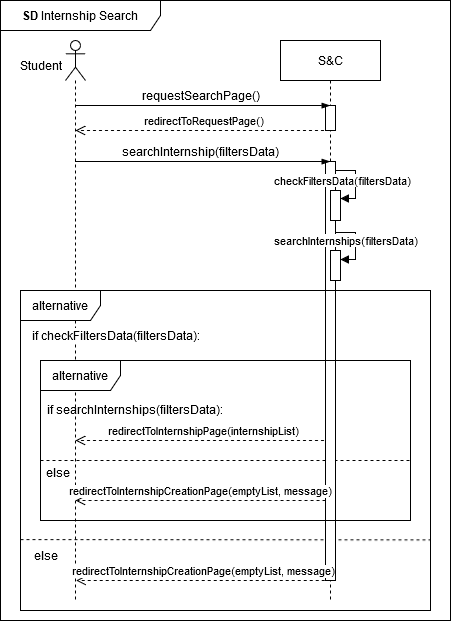
\includegraphics[width=1\textwidth]{RASD/Images/UseCases/US05_InternshipSearch.drawio.png}
                \label{fig:CompleteStudentProfile}
            \end{figure}
            
            % -- US6 --
            \newpage
            \item \textbf{Application for internship}
            
            \begin{longtable}{|l|p{11cm}|}  
                \hline
                \textbf{Name} & 
                    \textbf{Application for Internship} \\
                \hline
                
                \textbf{Actors} & 
                    \begin{enumerate}[label=\textbullet, itemsep=0em]
                        \item Student
                    \end{enumerate} \\
                \hline
                
                \textbf{Entry Condition} & 
                    \begin{enumerate}[label=\textbullet, itemsep=0em]
                        \item The student decides to apply to an internship;
                        \item The student has an account and is logged in;
                        \item The student searched an internship and he/she is on the dedicated page.
                    \end{enumerate} \\
                \hline
                
                \textbf{Event Flow} &
                    \begin{enumerate}[label=\arabic*., itemsep=0.2em]
                        \item The student presses the "Apply" button;
                        \item S\&C redirects the student to the page of the internship position;
                        \item The student can see all the information
                        \item The student has to accept terms and condition of the application
                        \item The student presses the "Confirm" button
                    \end{enumerate} \\
                \hline
                
                \textbf{Exit Condition} & 
                    The user sent the application and gets redirected to his own profile page\\
                \hline
                
                \textbf{Exceptions} &
                    \begin{enumerate}[label=\arabic*., itemsep=0.1em]
                        \item The application is made to an internship position who closed in the meanwhile but the front end has not yet rendered the change.
                            \begin{itemize}[label=\textbullet, itemsep=0em]
                                \item In that case, S\&C will display  warning message on the screen saying that the internship is not available.
                            \end{itemize}
                    \end{enumerate} \\
                \hline
            \end{longtable}
    
            \newpage
            \begin{figure}[h!]
                \centering   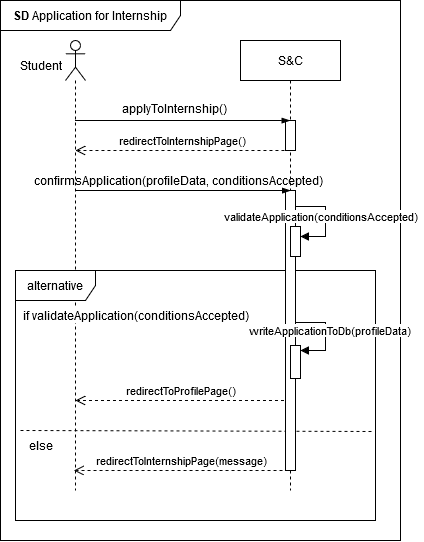
\includegraphics[width=1\textwidth]{RASD/Images/UseCases/US06_InternshipApplication.drawio.png}
                \label{fig: Application for Internship}
            \end{figure}

            % -- US7 --
            \newpage
            \item \textbf{Student Examines Applications} 
            \begin{longtable}{|l|p{11cm}|}  
                \hline
                \textbf{Name} & 
                    \textbf{Student Examines Applications} \\
                \hline
                
                \textbf{Actors} & 
                    \begin{enumerate}[label=\textbullet, itemsep=0em]
                        \item Student
                    \end{enumerate} \\
                \hline
                
                \textbf{Entry Condition} & 
                    \begin{enumerate}[label=\textbullet, itemsep=0em]
                        \item The student decides to examine its applications;
                        \item The student has an account and is logged in;
                        \item The student is on its profile page.
                    \end{enumerate} \\
                \hline
                
                \textbf{Event Flow} &
                    \begin{enumerate}[label=\arabic*., itemsep=0.2em]
                        \item The student presses the "Applications" button;
                        \item S\&C redirects the student to the page of the applications;
                        \item The student can click on any of them to get more details
                    \end{enumerate} \\
                \hline
                
                \textbf{Exit Condition} & 
                    The student exits his own profile page or confirms an application\\
                \hline
                
                \textbf{Exceptions} &
                    \begin{enumerate}[label=\arabic*., itemsep=0.1em]
                        \item The student doesn't have any applications
                            \begin{itemize}[label=\textbullet, itemsep=0em]
                                \item In that case, S\&C will display an empty list and a warning message on the screen saying that the student has not made any applications yet.
                            \end{itemize}
                    \end{enumerate} \\
                \hline
            \end{longtable}

            \newpage
            \begin{figure}[h!]
                \centering  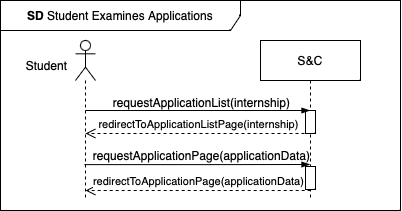
\includegraphics[width=1\textwidth]{RASD/Images/UseCases/US07_StudentExaminesApplications.drawio.png}
                \label{fig:example}
            \end{figure}
        \end{enumerate}

    % -----------------------------------
    \newpage
    \subsubsection{Company Use Cases}
        \begin{enumerate}[label=\textbf{[US\arabic*]}, left = 0pt, align = left, resume]
            % -- US8 --    
            \item \textbf{Company Registration}
        
            \begin{longtable}{|l|p{11cm}|}  
                \hline
                \textbf{Name} & 
                    \textbf{Company Registration} \\
                \hline
                
                \textbf{Actors} & 
                    \begin{enumerate}[label=\textbullet, itemsep=0em]
                        \item Company
                    \end{enumerate} \\
                \hline
                
                \textbf{Entry Condition} & 
                    The company does not have an account and is on the main page of S\&C. \\
                \hline
                
                \textbf{Event Flow} &
                    \begin{enumerate}[label=\arabic*., itemsep=0.2em]
                        \item The company presses the "Register as Company" button;
                        \item S\&C redirects the company to the register page;

                        \item The company enters the following information in the corresponding form field:
                        \begin{itemize}[label=\textbullet, itemsep=0em]
                            \item Company mail;
                            \item Password;
                            \item Confirm password
                            \item Company name;
                            \item Logo (not mandatory);
                            \item Short description of the company;
                            \item Location.
                        \end{itemize}
                        
                        \item The company presses the "Subscribe" button;
                        \item S\&C validates the data;
                        \item S\&C creates the company's account;
                        \item S\&C redirects the company to the homepage of S\&C.
                    \end{enumerate} \\
                \hline
                
                \textbf{Exit Condition} & 
                    The company's account is created, and it's logged in. \\
                \hline
                
                \textbf{Exceptions} &
                    \begin{enumerate}[label=\arabic*., itemsep=0.1em]
                        \item The company provides invalid data (e.g., invalid email format, duplicate email address, mismatched passwords).
                            \begin{itemize}[label=\textbullet, itemsep=0em]
                                \item S\&C validates the input and detects the invalid data.
                                \item S\&C displays an error message explaining the specific validation errors.
                                \item The company must correct the errors and resubmit the form.
                            \end{itemize}
                    \end{enumerate} \\
                \hline
                
            \end{longtable}

            \newpage
            \begin{figure}[h!]
                \centering  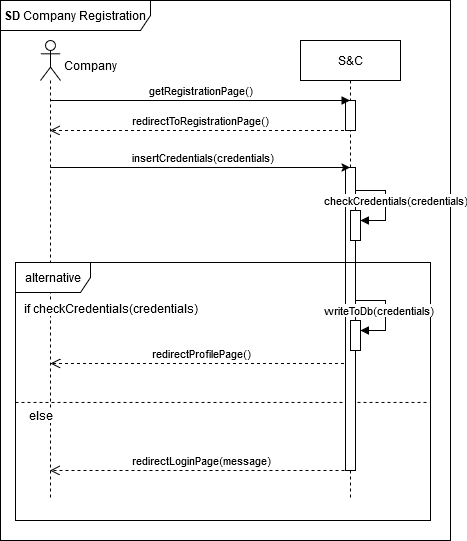
\includegraphics[width=1\textwidth]{RASD/Images/UseCases/US08_CompanyRegistration.drawio.png}
                \label{fig:CompanyRegistration}
            \end{figure}

            % -- US9 --
            \newpage
            \item \textbf{Post a new Internship}
            
            \begin{longtable}{|l|p{11cm}|}  
                \hline
                \textbf{Name} & 
                    \textbf{Post a new internship} \\
                \hline
                
                \textbf{Actors} & 
                    \begin{enumerate}[label=\textbullet, itemsep=0em]
                        \item Company;
                        \item Student.
                    \end{enumerate} \\
                \hline
                
                \textbf{Entry Condition} & 
                    The company has an account and is logged in. \\
                \hline
                
                \textbf{Event Flow} &
                    \begin{enumerate}[label=\arabic*., itemsep=0.2em]
                        \item The company presses the "Add New Internship" button;
                        \item S\&C displays a form that the company have to fill;
                        \item The company fills the form;
                        \item The company presses the "Publish" button;
                        \item S\&C validates the data;
                        \item S\&C displays a Success Message;
                        \item S\&C redirects the company to the main page;
                        \item S\&C identifies the students' profiles that match the internship based on skills, academic background, and location;
                        \item S\&C sends notifications to students that match offering the internship.
                    \end{enumerate} \\
                \hline
                
                \textbf{Exit Condition} & 
                    The company posts a new internship. \\
                \hline
                
                \textbf{Exceptions} &
                    \begin{enumerate}[label=\arabic*., itemsep=0.1em]
                        \item The company leaves one or more mandatory fields empty.
                            \begin{itemize}[label=\textbullet, itemsep=0em]
                                \item S\&C displays an error message indicating the missing fields.
                                \item S\&C highlights the empty fields in the form.
                                \item The company is prompted to complete the form before resubmitting.
                            \end{itemize}
                        \item The company provides invalid data (e.g., incorrect date formats, non-numeric salary inputs).
                            \begin{itemize}[label=\textbullet, itemsep=0em]
                                \item S\&C validates the input and detects the invalid data.
                                \item S\&C displays an error message explaining the specific validation errors.
                                \item The company must correct the errors and resubmit the form
                            \end{itemize}
                        \item The company is not logged in.
                            \begin{itemize}[label=\textbullet, itemsep=0em]
                                \item S\&C denies access and displays an error message: "You must be logged in with a company account to perform this action."
                                \item S\&C redirects the user to the login page.
                            \end{itemize}
                        \item The company attempts to post an internship with identical details to an already existing one.
                            \begin{itemize}[label=\textbullet, itemsep=0em]
                                \item S\&C detects the duplicate entry and displays a warning: "An internship with similar details already exists. Please review your submission."
                            \end{itemize}
                    \end{enumerate} \\
                \hline
                
            \end{longtable}

            \newpage
            \begin{figure}[h!]
                \centering  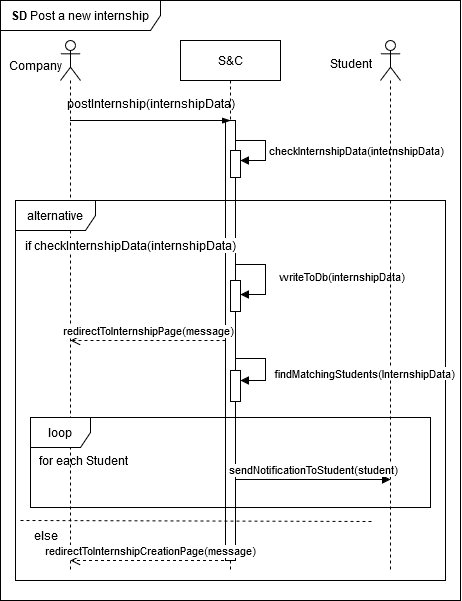
\includegraphics[width=1\textwidth]{RASD/Images/UseCases/US09_PostNewInternship.drawio.png}
                \label{fig:example}
            \end{figure}

            % -- US10 --       
            \newpage
            \item \textbf{Close an internship}
            
            \begin{longtable}{|l|p{11cm}|}  
                \hline
                \textbf{Name} & 
                    \textbf{Close an internship} \\
                \hline
                
                \textbf{Actors} & 
                    \begin{enumerate}[label=\textbullet, itemsep=0em]
                        \item Company
                    \end{enumerate} \\
                \hline
                
                \textbf{Entry Condition} & 
                    \begin{enumerate}[label=\textbullet, itemsep=0em]
                        \item The company has an account and is logged in;
                        \item The company has at least one open internship.
                    \end{enumerate} \\
                \hline 
                
                \textbf{Event Flow} &
                    \begin{enumerate}[label=\arabic*., itemsep=0.2em]
                        \item The company enters the open internship section;
                        \item The company chooses the internship they want to close;
                        \item The company presses the "Close" button;
                        \item S\&C validates the data;
                        \item S\&C displays a Success Message;
                        \item S\&C redirects the company to the main page;
                    \end{enumerate} \\
                \hline
                
                \textbf{Exit Condition} & 
                    The company posts a new internship. \\
                \hline
                
                \textbf{Exceptions} &
                    \begin{enumerate}[label=\arabic*., itemsep=0.1em]
                        \item The company is not logged in.
                            \begin{itemize}[label=\textbullet, itemsep=0em]
                                \item S\&C denies access and displays an error message: "You must be logged in with a company account to perform this action."
                                \item S\&C redirects the user to the login page.
                            \end{itemize}
                        \item The company provides invalid data (e.g., already closed internship, nonexistent internship).
                            \begin{itemize}[label=\textbullet, itemsep=0em]
                                \item S\&C validates the input and detects the invalid data.
                                \item S\&C displays an error message explaining the specific validation errors.
                            \end{itemize}
                    \end{enumerate} \\
                \hline
                
            \end{longtable}

            \newpage     
            \begin{figure}[h!]
                \centering  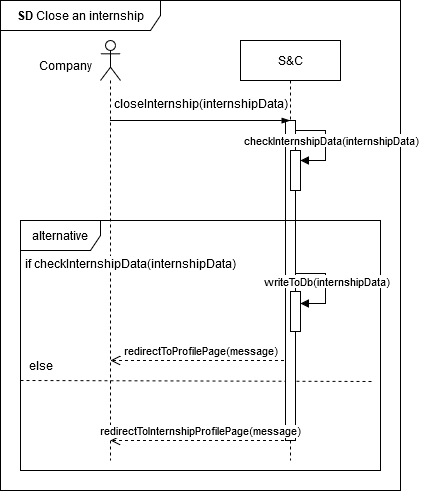
\includegraphics[width=1\textwidth]{RASD/Images/UseCases/US10_CloseInternship.drawio.png}
                \label{fig:example}
            \end{figure}
            
            % -- US11 --
            \newpage
            \item \textbf{Company Examines Internship Positions} 
            \begin{longtable}{|l|p{11cm}|}  
                \hline
                \textbf{Name} & 
                    \textbf{Company Examines Internship Positions} \\
                \hline
                
                \textbf{Actors} & 
                    \begin{enumerate}[label=\textbullet, itemsep=0em]
                        \item Company
                    \end{enumerate} \\
                \hline
                
                \textbf{Entry Condition} & 
                    \begin{enumerate}[label=\textbullet, itemsep=0em]
                        \item The company decides to examine its internship positions;
                        \item The company has an account and is logged in;
                        \item The company is on its profile page.
                    \end{enumerate} \\
                \hline
                
                \textbf{Event Flow} &
                    \begin{enumerate}[label=\arabic*., itemsep=0.2em]
                        \item The company presses the "Internships Positions" button;
                        \item S\&C redirects the company to the page of the internship positions;
                        \item The company can click on any of them to get more details;
                        \item For each internship position, the company can click on the "Candidate Matching" button;
                        \item S\&C displays a list of candidates who match the internship requirements;
                        \item The company can examine the list of candidates and review their profiles.
                    \end{enumerate} \\
                \hline
                
                \textbf{Exit Condition} & 
                    The company exits his own profile page or goes checking out some applications\\
                \hline
                
                \textbf{Exceptions} &
                    \begin{enumerate}[label=\arabic*., itemsep=0.1em]
                        \item The company doesn't have any  internship positions
                            \begin{itemize}[label=\textbullet, itemsep=0em]
                                \item In that case, S\&C will display an empty list and a warning message on the screen saying that the company has not  any internship positions yet.
                            \end{itemize}
                    \end{enumerate} \\
                \hline
            \end{longtable}

            \newpage
            \begin{figure}[h!]
                \centering
                    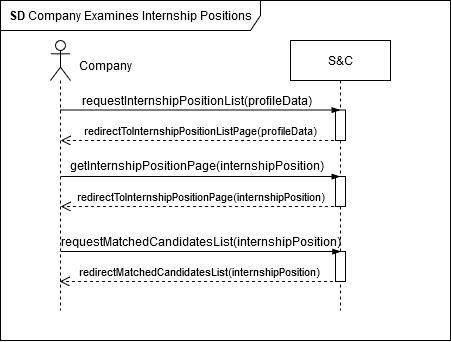
\includegraphics[width=1\textwidth]{RASD/Images/UseCases/US11_CompanyExaminesInternshipPositions.drawio.png}
                \label{fig:example}
            \end{figure}
            \newpage     

            % -- US12 --
            \newpage
            \item \textbf{Company Examines Internships} 
            
            \begin{longtable}{|l|p{11cm}|}  
                \hline
                \textbf{Name} & 
                    \textbf{Company Examines Internships} \\
                \hline
                
                \textbf{Actors} & 
                    \begin{enumerate}[label=\textbullet, itemsep=0em]
                        \item Company
                    \end{enumerate} \\
                \hline
                
                \textbf{Entry Condition} & 
                    \begin{enumerate}[label=\textbullet, itemsep=0em]
                        \item The company decides to examine its internships;
                        \item The company has an account and is logged in;
                        \item The company is on its profile page.
                    \end{enumerate} \\
                \hline
                
                \textbf{Event Flow} &
                    \begin{enumerate}[label=\arabic*., itemsep=0.2em]
                        \item The company presses the "Internships" button;
                        \item S\&C redirects the company to the page of the internships;
                        \item The company can click on any of them to get more details
                    \end{enumerate} \\
                \hline
                
                \textbf{Exit Condition} & 
                    The company exits his own profile page \\
                \hline
                
                \textbf{Exceptions} &
                    \begin{enumerate}[label=\arabic*., itemsep=0.1em]
                        \item The company doesn't have any  internships
                            \begin{itemize}[label=\textbullet, itemsep=0em]
                                \item In that case, S\&C will display an empty list and a warning message on the screen saying that the company has not  any internships yet.
                            \end{itemize}
                    \end{enumerate} \\
                \hline
            \end{longtable}

            \newpage
            \begin{figure}[h!]
                \centering  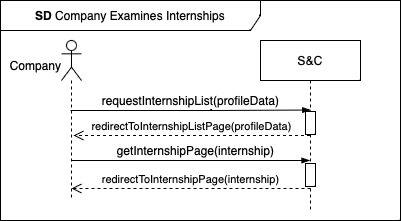
\includegraphics[width=1\textwidth]{RASD/Images/UseCases/US12_CompanyExaminesInternships.drawio.png}
                \label{fig:example}
            \end{figure}

            % -- US13 --
            \newpage
            \item \textbf{Company Examines Applications} 
            
            \begin{longtable}{|l|p{11cm}|}  
                \hline
                \textbf{Name} & 
                    \textbf{Company Examines Applications} \\
                \hline
                
                \textbf{Actors} & 
                    \begin{enumerate}[label=\textbullet, itemsep=0em]
                        \item Company
                    \end{enumerate} \\
                \hline
                
                \textbf{Entry Condition} & 
                    \begin{enumerate}[label=\textbullet, itemsep=0em]
                        \item The company decides to examine its applications;
                        \item The company has an account and is logged in;
                        \item The company is on its profile page.
                    \end{enumerate} \\
                \hline
                
                \textbf{Event Flow} &
                    \begin{enumerate}[label=\arabic*., itemsep=0.2em]
                        \item Included use case: Company Examines Internship Positions 
                        \item The company presses the "Applications" button;
                        \item S\&C redirects the company to the page of the applications;
                        \item The company can click on any of them to get more details
                    \end{enumerate} \\
                \hline
                
                \textbf{Exit Condition} & 
                    The company exits his own profile page or accept, refuse or request an assessment an application\\
                \hline
                
                \textbf{Exceptions} &
                    \begin{enumerate}[label=\arabic*., itemsep=0.1em]
                        \item The company doesn't have any applications for an internship position
                            \begin{itemize}[label=\textbullet, itemsep=0em]
                                \item In that case, S\&C will display an empty list and a warning message on the screen saying that the company has not  any applications for that internship yet.
                            \end{itemize}
                    \end{enumerate} \\
                \hline
            \end{longtable}
            
            \newpage           
            \begin{figure}[h!]
                \centering  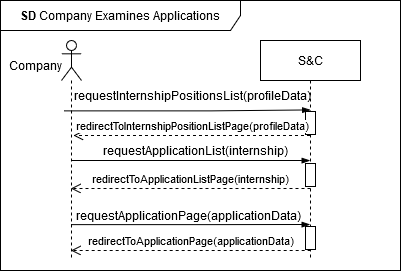
\includegraphics[width=1\textwidth]{RASD/Images/UseCases/US13_CompanyExaminesApplications.drawio.png}
                \label{fig:example}
            \end{figure}

            % -- US14 --        
            \newpage
            \item \textbf{Application Acceptance or Rejection}
            
            \begin{longtable}{|l|p{11cm}|}  
                \hline
                \textbf{Name} & 
                    \textbf{Application Acceptance or Rejection} \\
                \hline
                
                \textbf{Actors} & 
                    \begin{enumerate}[label=\textbullet, itemsep=0em]
                        \item Company
                    \end{enumerate} \\
                \hline
                
                \textbf{Entry Condition} & 
                    \begin{enumerate}[label=\textbullet, itemsep=0em]
                        \item The company has an account and is logged in;
                        \item The company knows which candidate to accept or reject; 
                        \item The company is in the dedicate page of an open internship that it has.
                    \end{enumerate} \\
                \hline
                
                \textbf{Event Flow} &
                    \begin{enumerate}[label=\arabic*., itemsep=0.2em]
                        \item The company clicks on the button to see the list of candidates;
                        \item The company can click on each item of the list to visit the profile page of the candidate;
                        \item The company clicks on the "Accept" or "Reject" button in correspondence with the candidate
                        \item S\&C displays a Success Message;
                    \end{enumerate} \\
                \hline
                
                \textbf{Exit Condition} & 
                    The candidate is accepted or rejected. \\
                \hline
                
                \textbf{Exceptions} &
                    \begin{enumerate}[label=\arabic*., itemsep=0.1em]
                        \item The company has no candidates for an open internship.
                            \begin{itemize}[label=\textbullet, itemsep=0em]
                                \item In that case, S\&C will show an empty list an display a notification which says no applications were found for that position.
                            \end{itemize}
                    \end{enumerate} \\
                \hline
            \end{longtable}

            \newpage
            \begin{figure}[h!]
                \centering  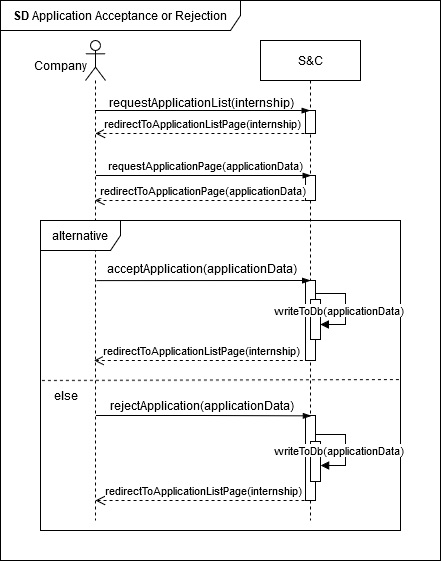
\includegraphics[width=1\textwidth]{RASD/Images/UseCases/US14_ApplicationAcceptanceRejection.drawio.png}
                \label{fig:example}
            \end{figure}

            % -- US15 --
            \newpage
            \item \textbf{Further Assessment for Application}
            
            \begin{longtable}{|l|p{11cm}|}  
                \hline
                \textbf{Name} & 
                    \textbf{Further Assessment for Application} \\
                \hline
                
                \textbf{Actors} & 
                    \begin{enumerate}[label=\textbullet, itemsep=0em]
                        \item Company
                    \end{enumerate} \\
                \hline
                
                \textbf{Entry Condition} & 
                    \begin{enumerate}[label=\textbullet, itemsep=0em]
                        \item The company has an account and is logged in;
                        \item The company knows which candidates have to undergo more assessment before being accepted or rejected;
                        \item The company is in the dedicate page of an open internship that it has.
                    \end{enumerate} \\
                \hline
                
                \textbf{Event Flow} &
                    \begin{enumerate}[label=\arabic*., itemsep=0.2em]
                        \item The company clicks on the button to see the list of candidates;
                        \item The company can click on each item of the list to visit the profile page of the candidate;
                        \item The company clicks the "Assess Further" button in correspondence with the candidate;
                        \item The company is prompted a calendar to choose when to schedule the interview and an input field to put the link of the online room;
                        \item The company confirms the date;
                        \item S\&C displays a Success Message.
                    \end{enumerate} \\
                \hline
                
                \textbf{Exit Condition} & 
                    The company has scheduled a new interview. \\
                \hline
                
                \textbf{Exceptions} &
                    \begin{enumerate}[label=\arabic*., itemsep=0.1em]
                        \item The company has no candidates for an open internship.
                            \begin{itemize}[label=\textbullet, itemsep=0em]
                                \item In that case, S\&C will show an empty list and display a notification which says no applications were found for that position.
                            \end{itemize}                           
                        \item The company inserted an invalid link.
                            \begin{itemize}[label=\textbullet, itemsep=0em]
                                \item S\&C validates the input and detects the invalid data.
                                \item S\&C displays an error message explaining the specific validation error.
                            \end{itemize}
                            
                    \end{enumerate} \\
                \hline
            \end{longtable}
            
            \newpage
            \begin{figure}[h!]
                \centering  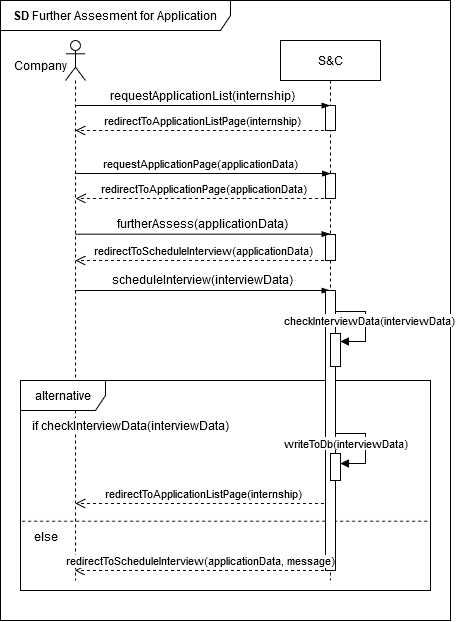
\includegraphics[width=1\textwidth]{RASD/Images/UseCases/US15_FurtherAssessment.drawio.png}
                \label{fig:example}
            \end{figure}
            
        \end{enumerate}

    % -----------------------------------
    \newpage
    \subsubsection{Users (Company and Student) Use Cases}
    Notice that in this subsection when we refer to users we intend students and companies only.
        \begin{enumerate}[label=\textbf{[US\arabic*]}, left = 0pt, align = left, resume]
            % -- US16 --
            \item \textbf{Feedback from User}
            
            \begin{longtable}{|l|p{11cm}|}  
                \hline
                \textbf{Name} & 
                    \textbf{Feedback from User} \\
                \hline
                
                \textbf{Actors} & 
                    \begin{enumerate}[label=\textbullet, itemsep=0em]
                        \item User
                    \end{enumerate} \\
                \hline
                
                \textbf{Entry Condition} & 
                    \begin{enumerate}[label=\textbullet, itemsep=0em]
                        \item The user has an account and is logged in;
                        \item The user has participated in the internship;
                        \item The internship has finished.
                    \end{enumerate} \\
                \hline
                
                \textbf{Event Flow} &
                    \begin{enumerate}[label=\arabic*., itemsep=0.2em]
                        \item The user navigates to the page of the just finished internship;
                        \item The user clicks the button to create a feedback;
                        \item The user inserts a rating and a comment;
                        \item The user sends it by clicking "Send";
                        \item S\&C validates the data;
                        \item S\&C displays a Success Message.
                    \end{enumerate} \\
                \hline
                
                \textbf{Exit Condition} & 
                    The feedback is sent and the user is redirected to the application page \\
                \hline

                \textbf{Exceptions} &
                    \begin{enumerate}[label=\arabic*., itemsep=0.1em]
                        \item The user provides invalid data (e.g., rating outside the range).
                            \begin{itemize}[label=\textbullet, itemsep=0em]
                                \item S\&C validates the input and detects the invalid data.
                                \item S\&C displays an error message explaining the specific validation errors.
                            \end{itemize}
                    \end{enumerate} \\
                \hline
            \end{longtable}

            \newpage
            \begin{figure}[h!]
                \centering  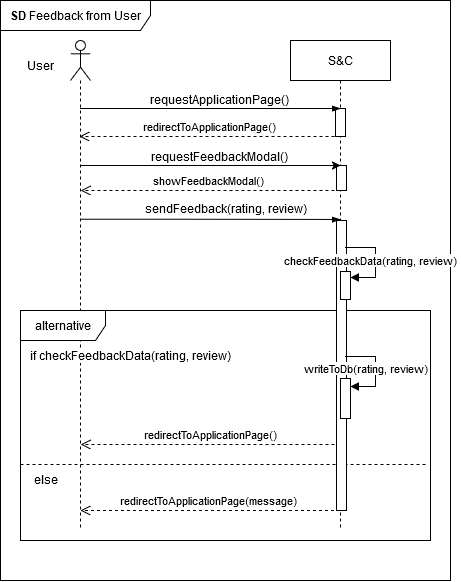
\includegraphics[width=1\textwidth]{RASD/Images/UseCases/US16_FeedbackFromUser.drawio.png}
                \label{fig:example}
            \end{figure}

            % -- US17 --
            \newpage
            \item \textbf{Communication between Users}
            
            \begin{longtable}{|l|p{11cm}|}  
                \hline
                \textbf{Name} & 
                    \textbf{Communication between Users} \\
                \hline
                
                \textbf{Actors} & 
                    \begin{enumerate}[label=\textbullet, itemsep=0em]
                        \item User
                    \end{enumerate} \\
                \hline
                
                \textbf{Entry Condition} & 
                    \begin{enumerate}[label=\textbullet, itemsep=0em]
                        \item The user has an account and is logged in;
                        \item The user is participating in the internship;
                        \item A user has to communicate something while an internship is ongoing.
                    \end{enumerate} \\
                \hline
                
                \textbf{Event Flow} &
                    \begin{enumerate}[label=\arabic*., itemsep=0.2em]
                        \item The user navigates to the page of the ongoing internship;
                        \item The user clicks the button to create a new complaint or a new suggestion;
                        \item The user inserts a message and sends it; 
                    \end{enumerate} \\
                \hline
                
                \textbf{Exit Condition} & 
                    The suggestion/complaint is sent and the student/company is redirected to the application page \\
                \hline
                \hline
            \end{longtable}

            \newpage
            \begin{figure}[h!]
                \centering  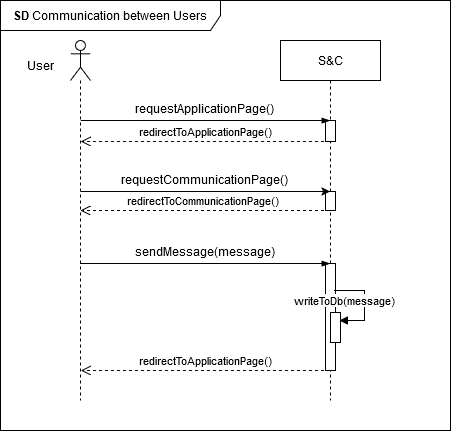
\includegraphics[width=1\textwidth]{RASD/Images/UseCases/US17_CommunicationBetweenUsers.drawio.png}
                \label{fig:example}
            \end{figure}

        \end{enumerate}

    % -----------------------------------
    \newpage
    \subsubsection{Universities Use Cases}
        \begin{enumerate}[label=\textbf{[US\arabic*]}, left = 0pt, align = left, resume]
            % -- US18 --    
            \item \textbf{University Registration}
        
            \begin{longtable}{|l|p{11cm}|}  
                \hline
                \textbf{Name} & 
                    \textbf{University Registration} \\
                \hline
                
                \textbf{Actors} & 
                    \begin{enumerate}[label=\textbullet, itemsep=0em]
                        \item University
                    \end{enumerate} \\
                \hline
                
                \textbf{Entry Condition} & 
                    The university does not have an account and is on the main page of S\&C. \\
                \hline
                
                \textbf{Event Flow} &
                    \begin{enumerate}[label=\arabic*., itemsep=0.2em]
                        \item The university presses the "Register as University" button;
                        \item S\&C redirects the university to the register page;

                        \item The university enters the following information in the corresponding form field:
                        \begin{itemize}[label=\textbullet, itemsep=0em]
                            \item University mail;
                            \item Password;
                            \item Confirm password
                            \item University name;
                            \item Address;
                            \item URL of it's website.
                        \end{itemize}
                        
                        \item The university presses the "Subscribe" button;
                        \item S\&C validates the data;
                        \item S\&C creates the university's account;
                        \item S\&C redirects the university to the homepage of S\&C.
                    \end{enumerate} \\
                \hline
                
                \textbf{Exit Condition} & 
                    The university's account is created, and it's logged in. \\
                \hline
                
                \textbf{Exceptions} &
                    \begin{enumerate}[label=\arabic*., itemsep=0.1em]
                        \item The university provides invalid data (e.g., invalid email format, duplicate email address, mismatched passwords).
                            \begin{itemize}[label=\textbullet, itemsep=0em]
                                \item S\&C validates the input and detects the invalid data.
                                \item S\&C displays an error message explaining the specific validation errors.
                                \item The university must correct the errors and resubmit the form.
                            \end{itemize}
                    \end{enumerate} \\
                \hline
                
            \end{longtable}

            \newpage
            \begin{figure}[h!]
                \centering  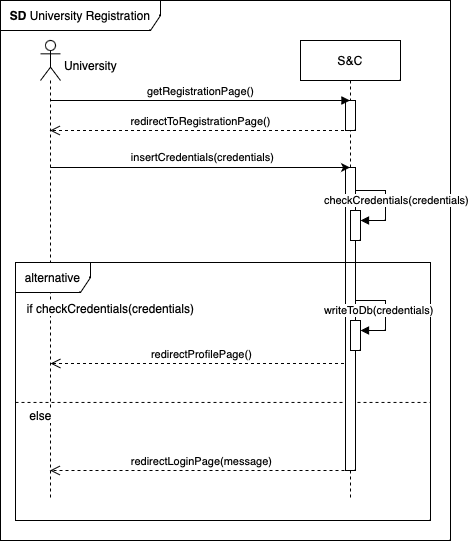
\includegraphics[width=1\textwidth]{RASD/Images/UseCases/US18_UniversityRegistration.drawio.png}
                \label{fig:example}
            \end{figure}
            
            % -- US19 --
            \newpage
            \item \textbf{University Monitors Internships}
            
            \begin{longtable}{|l|p{11cm}|}  
                \hline
                \textbf{Name} & 
                    \textbf{University Monitors Internships} \\
                \hline
                
                \textbf{Actors} & 
                    University \\
                \hline
                
                \textbf{Entry Condition} & 
                    The university is logged in \\
                \hline
                
                \textbf{Event Flow} &
                    \begin{enumerate}[label=\arabic*., itemsep=0.2em]
                        \item The university has a list of internships done by its students on its home page;
                        \item The university can click on any of them to get more details;
                    \end{enumerate} \\
                \hline
                
                \textbf{Exit Condition} & 
                    The university stops scrolling the list of hits students who got an internship  profile. \\
                \hline
                
                \textbf{Exceptions} &
                    \begin{enumerate}[label=\arabic*., itemsep=0.1em]
                        \item The universities has no students who got an internship.
                            \begin{itemize}[label=\textbullet, itemsep=0em]
                                \item In that case, S\&C will display a message on the screen saying that no enrolled student got any internship.
                            \end{itemize}
                    \end{enumerate} \\
                \hline
                
            \end{longtable}

            \newpage
            \begin{figure}[h!]
                \centering  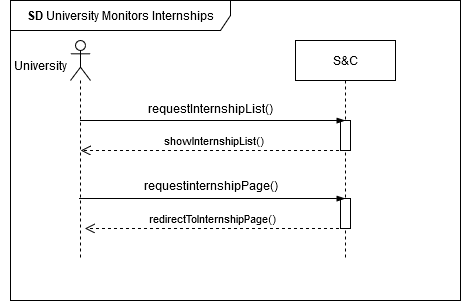
\includegraphics[width=1\textwidth]{RASD/Images/UseCases/US19_UniversityMonitorsInternships.drawio.png}
                \label{fig:example}
            \end{figure}

        \end{enumerate}
        
\newpage

\subsection{Requirement Mapping}

\begin{enumerate}[label={[G\arabic*]}]
\item \textbf{Internship Lookup for Students}: 
                Help students in their search for an internship by connecting their profiles with well-suited internship offers from companies.

\begin{longtable}{|p{8cm}|p{8cm}|}
\hline
\rowcolor[HTML]{CFE2F3} 
\textbf{Requirements} & \textbf{Mapped To} \\
\hline
\endfirsthead

\hline
\endfoot

\hline
\endlastfoot
R1 S\&C shall allow users to sign up. & D1 Students insert correct information about their skills and experience \\
R2 S\&C shall allow users to fill their profile information on sign up & D2 Students apply to jobs in countries where they have a work permit \\
R3 S\&C shall allow users to log in. & D3 Companies offer existing and legal contracts for the internships \\
R4 S\&C shall allow users to log out. & D4 Companies insert correct information about the internships \\
R5 S\&C shall allow users to update their profile information. & D5 Companies periodically review information about the internship candidates \\
R7 S\&C shall allow users to examine open internship positions.  & \\
R9 S\&C shall allow students to search for a specific kind of internship.  & \\ 
R10 S\&C shall allow students to apply for an internship.     & \\
R11 If an internship position suited to a student is opened, S\&C shall notify the student & \\
R12 When a student issues a search for an internship, S\&C shall list the different positions aligned with the student's profile.  & \\

\end{longtable}


\newpage
\item \textbf{Visibility for Internship Positions of the Companies}: 
                Allow companies to promote their internship positions to students and inform them about the availability of eligible candidates.
\begin{longtable}{|p{8cm}|p{8cm}|}
\hline
\rowcolor[HTML]{CFE2F3} 
\textbf{Requirements} & \textbf{Mapped To} \\
\hline
\endfirsthead

\hline
\endfoot

\hline
\endlastfoot
R1 S\&C shall allow users to sign up. & D1 Students insert correct information about their skills and experience \\
R2 S\&C shall allow users to fill their profile information on sign up & D2 Students apply to jobs in countries where they have a work permit \\
R3 S\&C shall allow users to log in. & D3 Companies offer existing and legal contracts for the internships \\
R4 S\&C shall allow users to log out. & D4 Companies insert correct information about the internships \\
R5 S\&C shall allow users to update their profile information. & D5 Companies periodically review information about the internship candidates \\
R7 S\&C shall allow users to examine open internship positions.  & \\
R9 S\&C shall allow students to search for a specific kind of internship.  & \\ 
R10 S\&C shall allow students to apply for an internship. & \\
R11 If an internship position suited to a student is opened, S\&C shall notify the student & \\
R12 When a student issues a search for an internship, S\&C shall list the different positions aligned with the student's profile.  & \\
R18 S\&C shall allow companies to open and examine its internship positions. & \\
\newpage
\end{longtable}
\item \textbf{Selection Process Management}: 
                Support the interaction and selection by providing a platform to companies to set up and conduct interviews, gather structured information about students and finalize the selections.

\begin{longtable}{|p{8cm}|p{8cm}|}
\hline
\rowcolor[HTML]{CFE2F3} 
\textbf{Requirements} & \textbf{Mapped To} \\
\hline
\endfirsthead

\hline
\endfoot

\hline
\endlastfoot

R1 S\&C shall allow users to sign up. & D1 Students insert correct information about their skills and experience \\
R2 S\&C shall allow users to fill their profile information on sign up & D2 Students apply to jobs in countries where they have a work permit \\
R3 S\&C shall allow users to log in. & D3 Companies offer existing and legal contracts for the internships \\
R4 S\&C shall allow users to log out. & D4 Companies insert correct information about the internships \\
R5 S\&C shall allow users to update their profile information. & D5 Companies periodically review information about the internship candidates \\
R8 S\&C shall allow users to examine their own applications. & \\
R10 S\&C shall allow students to apply for an internship.     & \\
R13 If an application has been accepted by a company, S\&C shall allow the student who made the application to confirm or refuse the internship & \\
R14 If a company signals that it needs an assessment of the students' skills, S\&C shall allow the student to schedule the quiz & \\
R15 After an assessment has been scheduled, S\&C shall allow the student to access the link and see the date of the assessment & \\
R16 S\&C shall allow the student to see the status of its applications & \\
R17 S\&C shall allow companies to accept or reject applications to their internship positions & \\
R18 S\&C shall allow companies to open and examine its internship positions. & \\
R19 S\&C shall allow companies to close internship positions. & \\
\end{longtable}
\newpage
\item \textbf{Data Collection for Recommendation System}: 
                Collect statistics in order to allow the efficiency of the matchmaking process of the recommendation system 


\begin{longtable}{|p{8cm}|p{8cm}|}
\hline
\rowcolor[HTML]{CFE2F3} 
\textbf{Requirements} & \textbf{Mapped To} \\
\hline
\endfirsthead

\hline
\endfoot

\hline
\endlastfoot
R1 S\&C shall allow users to sign up. & D1 Students insert correct information about their skills and experience \\
R2 S\&C shall allow users to fill their profile information on sign up & D2 Companies insert correct information about the internships \\
R3 S\&C shall allow users to log in. & D3 Students provide valuable feedback when asked for it \\
R4 S\&C shall allow users to log out. & \\
R5 S\&C shall allow users to update their profile information. & \\
R21 S\&C shall allow companies to leave private notes to students who are carrying out an internship with it & \\
R22 S\&C shall allow companies to send news about the internship to students who are carrying it out & \\
R23 S\&C shall allow both parties to communicate problems in a specific space of the website & \\
R24 S\&C shall allow students who took an internship with a company to rate the internship and vice versa & \\
R25 S\&C shall allow students who took an internship with a company to give suggestions to the company and vice versa & \\
R26 S\&C shall allow companies to send news about the internship to students who are carrying it out & \\
R27 S\&C shall allow both parties involved in an internship to communicate problems in a dedicated space & \\

\end{longtable}
\newpage
\item \textbf{Enhance Communication}: 
                Enhance communication between students and companies, through a shared space where they can exchange information, raise problems and collect complaints about the internships

\begin{longtable}{|p{8cm}|p{8cm}|}
\hline
\rowcolor[HTML]{CFE2F3} 
\textbf{Requirements} & \textbf{Mapped To} \\
\hline
\endfirsthead

\hline
\endfoot

\hline
\endlastfoot
R1 S\&C shall allow users to sign up. &  D5 Students provide valuable feedback when asked for it \\
R2 S\&C shall allow users to fill their profile information on sign up & D7 Companies provide valuable feedback when asked for it \\
R3 S\&C shall allow users to log in. & D8 Students raise problems through the platform \\
R4 S\&C shall allow users to log out. &  D9 Companies use the platform as principal mean of communication regarding the internships \\
R21 S\&C shall allow companies to leave private notes to students who are carrying out an internship with it & \\
R22 S\&C shall allow companies to send news about the internship to students who are carrying it out &  \\
R23 S\&C shall allow both parties to make complaints in a specific space of the website & \\
R24 S\&C shall allow students who took an internship with a company to rate the internship and vice versa &  \\
R25 S\&C shall allow students who took an internship with a company to give suggestions to the company and vice versa & \\
R26 S\&C shall allow companies to send news about the internship to students who are carrying it out & \\
R27 S\&C shall allow both parties involved in an internship to communicate problems in a dedicated space & \\
\end{longtable}
\item \textbf{Monitoring of Internships by Universities}: 
    Allow universities to see the situation of the internships of their students, including the complaints about them.

\begin{longtable}{|p{8cm}|p{8cm}|}
\hline
\rowcolor[HTML]{CFE2F3} 
\textbf{Requirements} & \textbf{Mapped To} \\
\hline
\endfirsthead

\hline
\endfoot

\hline
\endlastfoot
R1 S\&C shall allow users to sign up. & D10 Universities must register on the platform before their students can create accounts, as students are required to link their profiles to their university \\
R2 S\&C shall allow users to fill their profile information on sign up & \\
R3 S\&C shall allow users to log in. &  \\
R4 S\&C shall allow users to log out. & \\
R5 S\&C shall allow users to update their profile information. & \\
R28 S\&C shall allow universities to monitor the status of the internship of their students &  \\ 
R29 S\&C shall allow universities to see details of the internships of their students & \\

\end{longtable}
\end{enumerate}
\subsection{Performance Requirements}
S\&C has to guarantee certain performance requirements in order to fulfill the goals for which it has been designed. 
\begin{itemize}
    \item \textbf{Up-time}: it has to be at least 99.5\%, which is pretty standard.
    \item \textbf{Response time}: it has to be reasonable. Here we tend not to quantify too much the response time because it also depends on the type of connection the user has not only on how the platform is built. We would like the system to reflect changes in almost real-time.
    \item \textbf{Notifications}: they have to be delivered in a reasonable time. Again as above.
    \item \textbf{Scalability}: the platform must support busy periods as well as periods with less interactions.
\end{itemize}


\subsection{Design Constraints}
\subsubsection{Standard Compliance}
S\&C should be perfectly compliant with data regulations present in the countries in which it operates. Since it is supposed to work mainly in the EU, it should be compliant with GDPR rules and the recommendation system used to match students and companies if enhanced by AI should be compliant with the AI Act. Privacy is of paramount importance to the platform, therefore a series of legal contracts regulate the information that the users store into the platform and users have to accept the privacy policy before registering to the website. Moreover, the infrastructure of the website is designed to be secure and avoid any kind of data breach that could harm the privacy of the users registered to the platform.

\subsubsection{Hardware Limitations}
The hardware necessary for this kind of applications is barely minimum, indeed any computing device with internet access on the market can navigate the web and visit the website page of S\&C. However, the only important hardware limitation is having a big screen. Indeed the application will be available only for desktop view. Therefore a mobile phone (even with internet access) won't be capable of seeing the platform and interact with it.

\subsubsection{Any Other Constraint}
As long as inclusive support is concerned, S\&C has not already support for blind people, but it does not use any kind of audio support therefore it can be used by hearing-impaired people.

\subsection{Software System Attributes}
The software system attributes along with the design choices we made to enforce those attributes will be more documented in the DD in the corresponding section. In this section our goal is to give a general idea of their scope within our platform.

\subsubsection{Reliability}
S\&C must be reliable at all times. It has to be up and running continuously to provide users with a nice and fluid experience. The system should enforce data consistency which is a key component of reliability. 

\subsubsection{Availability}
Availability is of crucial importance to the platform. Indeed crashes and service interruptions should be avoided as much as possible. Maintenance must be scheduled and users must be alerted in advance when the website will not be available due to it.

\subsubsection{Security}
S\&C should be strongly secure. Requests should be validated on both the back-end and on the front-end side to ensure no malicious code will reach the data stored. Password encryption will keep securely stored the password of the users. The website will be protected by using specific libraries from cross-site request forgery attacks. User session should be managed in order to guarantee an adequate level of security.

\subsubsection{Maintainability}
The software of S\&C shall be as easy as possible to maintain. The code should be commented extensively for making new programmers who contribute to the development of the project aware of how all the function and components work. When possible, writing reusable code is preferred and, of course, modular programming is preferred over a monolithic style. Other techniques that will be used to make sure the system is going to be maintainable is to define clear boundaries between modules and apply as much decoupling among them as possible. The software of S\&C must be linked to a versioning control software to keep track of the changes made and by who they were made.

% \subsubsection{Portability} not necessary

% I merged the 2 use cases into 1
            % % -- US16 --
            % \item \textbf{Further Assessment for Application}
            
            % \begin{longtable}{|l|p{11cm}|}  
            %     \hline
            %     \textbf{Name} & 
            %         \textbf{Further Assessment for Application} \\
            %     \hline
                
            %     \textbf{Actors} & 
            %         Company\\
            %     \hline
                
            %     \textbf{Entry Condition} & 
            %         The company knows which candidates have to undergo more assessment before being accepted or rejected \\
            %     \hline
                
            %     \textbf{Event Flow} &
            %         \begin{enumerate}[label=\arabic*., itemsep=0.2em]
            %             \item Included use case: Company Login
            %             \item The company goes to the page of an open internship it has;
            %             \item The company clicks on the button to see the list of candidates;
            %             \item The company can click on each item of the list to visit the profile page of the candidate;
            %             \item The company clicks "Assess Further" 
            %             \item Included use case: Create assessment 
            %         \end{enumerate} \\
            %     \hline
                
            %     \textbf{Exit Condition} & 
            %         The candidate is notified that he has to undergo a phase of assessment. \\
            %     \hline
                
            %     \textbf{Exceptions} &
            %         \begin{enumerate}[label=\arabic*., itemsep=0.1em]
            %             \item The company has no candidates for an open internship.
            %                 \begin{itemize}[label=\textbullet, itemsep=0em]
            %                     \item In that case, S\&C will show an empty list and display a notification which says no applications were found for that position.
            %                 \end{itemize}
            %         \end{enumerate} \\
            %     \hline
            % \end{longtable}

            % % -- US17 --
            % \newpage
            % \item \textbf{Request Assessment}
            
            % \begin{longtable}{|l|p{11cm}|}  
            %     \hline
            %     \textbf{Name} & 
            %         \textbf{Request Assessment} \\
            %     \hline
                
            %     \textbf{Actors} & 
            %         Company, Student\\
            %     \hline
                
            %     \textbf{Entry Condition} & 
            %         The company pressed the button "Request Assessment" on an application \\
            %     \hline
                
            %     \textbf{Event Flow} &
            %         \begin{enumerate}[label=\arabic*., itemsep=0.2em]
            %             \item The company is prompted a calendar to choose when to schedule the interview and an input field to put the link of the online room
            %             \item After confirming the decision, the company is redirected to the page of the internship needing the assessment;
            %             \item From now on it will be able to accept or reject the student;
            %             \item The company clicks "Create Assessment" 
            %         \end{enumerate} \\
            %     \hline
                
            %     \textbf{Exit Condition} & 
            %         The assessment for the student has been created. \\
            %     \hline
                
            %     \textbf{Exceptions} &
            %         \begin{enumerate}[label=\arabic*., itemsep=0.1em]
            %             \item The company inputs the wrong date.
            %                 \begin{itemize}[label=\textbullet, itemsep=0em]
            %                     \item In that case, the company will have to inform the student with a different communication mean (e. g. by email)
            %                 \end{itemize}
            %             \item The company inserted the wrong link.
            %             \begin{itemize}[label=\textbullet, itemsep=0em]
            %             \item In that case, the company will have to inform the student with a different communication mean (e. g. by email)
            %             \end{itemize}
            %         \end{enumerate} \\
            %     \hline
            % \end{longtable}
